\documentclass[12pt,authoryear]{elsarticle}

%removed 'preprint submitted to elsevier
\makeatletter
\def\ps@pprintTitle{%
	\let\@oddhead\@empty
	\let\@evenhead\@empty
	\def\@oddfoot{\centerline{\thepage}}%
	\let\@evenfoot\@oddfoot}
\makeatother


\usepackage{graphicx}
\usepackage{background}
\backgroundsetup{opacity=.15,contents={
\includegraphics[scale=0.05]{IITR_new_logo_gray.png}}}

\usepackage{tfrupee}
\usepackage{subfigure}% Support for small, `sub' figures and tables

\usepackage{hyperref}
\hypersetup{
	pdftitle={ShortTitle},
	colorlinks=true,
	linkcolor=blue,
	citecolor=blue
}

\usepackage[a4paper,left=2.5cm,right=2.5cm,top=2.5cm,bottom=2.5cm]{geometry}

\usepackage{lscape}

\usepackage{url}
\usepackage{doi}
\urlstyle{same}

\usepackage{multicol}
\usepackage{multirow}
\usepackage{booktabs}

\usepackage{paralist} % in para list

\usepackage{lineno}

\makeatletter
\def\els@aparagraph[#1]#2{\elsparagraph[#1]{#2}}
\def\els@bparagraph#1{\elsparagraph*{#1}}
\makeatother

\newcommand{\colortableformat}{
	\renewcommand{\arraystretch}{1.3}
	\footnotesize
}

\usepackage[]{todonotes}
%\usepackage[disable]{todonotes}
\newcommand{\amit}[2][]
{\todo[inline,caption={}, size=\scriptsize,
	color=yellow!30, #1]{\renewcommand{\baselinestretch}{0.5}\selectfont#2 AA\par}}
\newcommand{\nidhi}[2][]

\def\mnote#1{\smallskip\centerline{\hfill{\sf\footnotesize\textcolor{blue}{#1}}}}
%\def\mnote#1{\relax}

\usepackage[capitalise,noabbrev]{cleveref}

\begin{document}
	
\begin{frontmatter}
	\title{\textbf{Here is a Title}}
	
	\author{First Author}
	\ead{fauthor@ce.iitr.ac.in}
	
	\author{Second Author\corref{cor}}
	\ead{sauthor@hotmail.com}
	
	\cortext[cor]{Corresponding author}
	
	\address{
		Department of Civil Engineering\\
		Indian Institute of Technology (IIT) Roorkee, Roorkee-247667, India\\
	}
	
	\begin{abstract}
		Collecting traffic da...
	\end{abstract}
%
\begin{keyword}
	traffic survey \sep household survey \sep trip diaries \sep activity-trip chain \sep person trip survey \sep crowd-sourced web survey
\end{keyword}
	
\end{frontmatter}

\linenumbers

%================================================
\section{Introduction} 
\label{sec:intro}
%================================================
%
\mnote{Traffic surveys and need}


%
\mnote{structure of the paper} 

To begin, this study provides a review of the existing literature related \citep{Census2011Jaipur} ...




%================================================
\section{Literature Review} 
\label{sec:Literature Review}
%================================================


\mnote{research gap}
From the foregoing discussion, it is clear that different survey ...


\citet{Agarwal2017PhD,AgarwalEtc2019PatnaIncomeBasedCadytsCalibration}
%
%================================================
\section{Countermeasures} 
\label{sec:approach}
%================================================
%
%================================================
\subsection{Coverage}
%================================================
%
As discussed in the previous section,
%
This highlights the feasibility of better cove...
\begin{figure}[!ht]
	\centering
	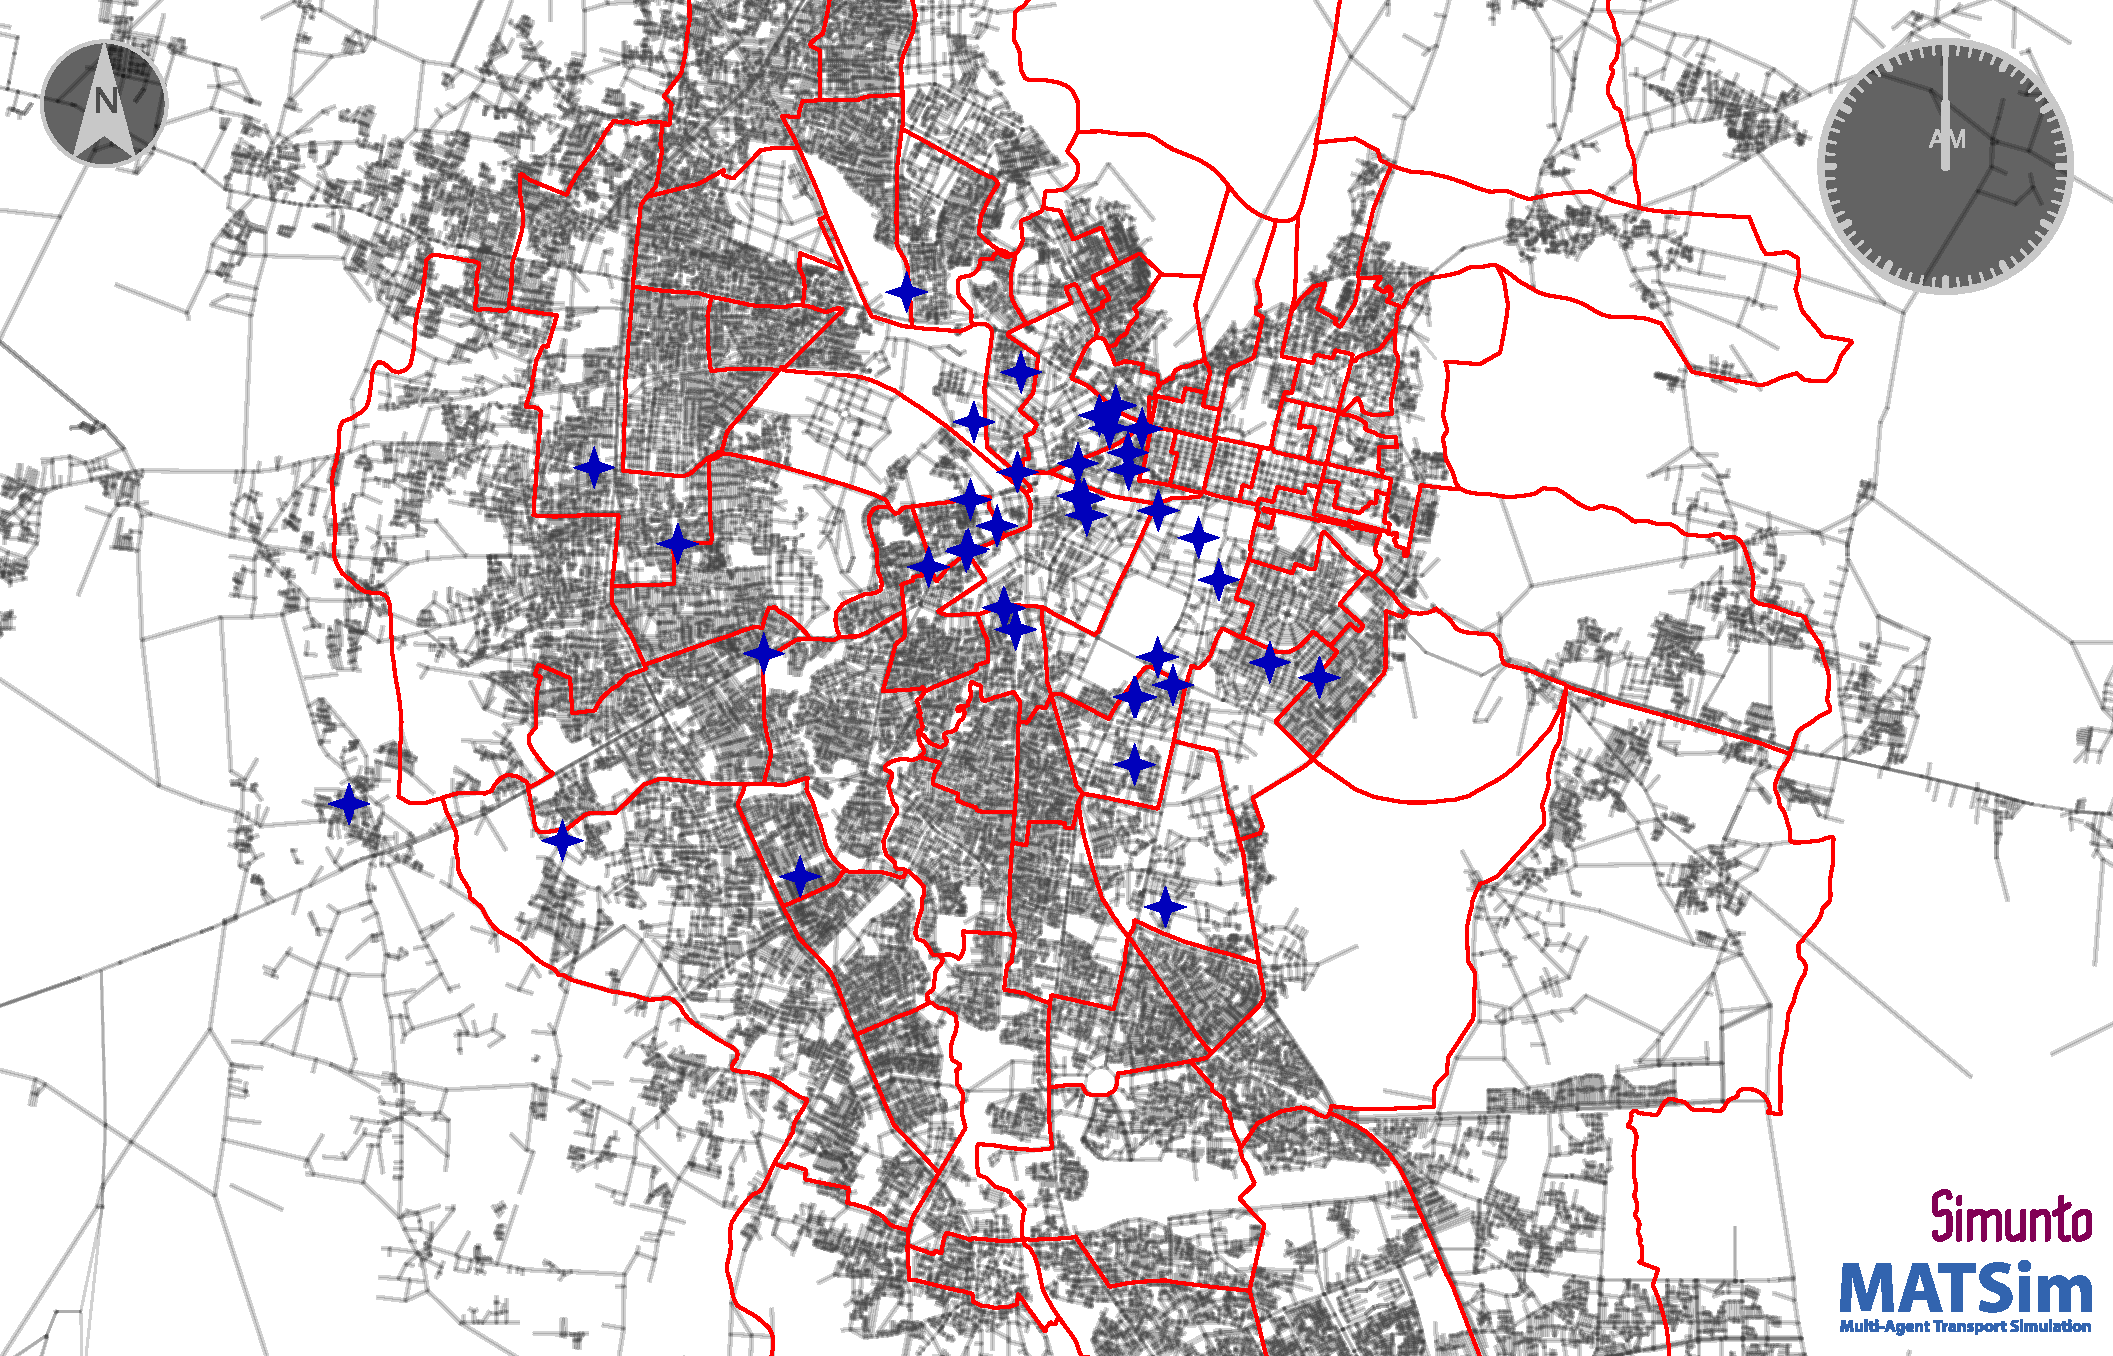
\includegraphics[trim=100 70 230 40, clip, width=0.7\linewidth]{insti_colleges_jaipur}
	\caption{Jaipur road network (in gray), ward (zone) boundaries (in red) and locations of institutes and colleges (in blue)}
	\label{fig:insticollegesjaipur}
\end{figure}

%================================================
\subsection{Collection of data using web-based self-completion and person-interview survey}
%================================================


%
%
%================================================
\section{TSaaS: Traffic Survey as a Service}
\label{sec:results}
%================================================
%
%================================================
\subsection{Overview}
%================================================


\begin{figure}[!ht]
	\centering
	\subfigure[
	\label{fig:startPage_demo}
	Start page for demo survey]
	{\resizebox*{4.5cm}{!}{
			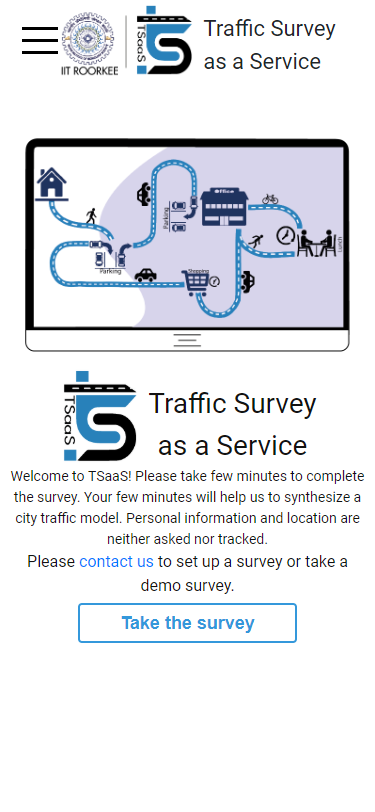
\includegraphics[trim=0 100 0 0,clip,width=\linewidth]{startPage_demo}}}
	\subfigure[
	\label{fig:startPage_insti}
	Start page for IIT Roorkee]
	{\resizebox*{4.5cm}{!}{
			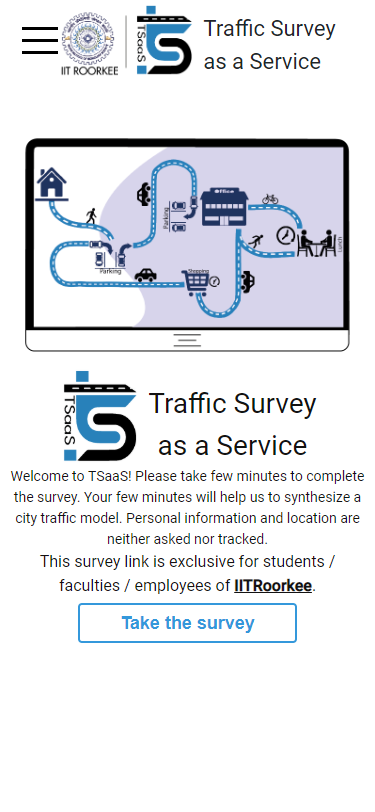
\includegraphics[trim=0 100 0 0,clip,width=\linewidth]{startPage_iitr}}}
	\caption{Start pages for demo survey and configured for the students / faculties of IIT Roorkee.}
	\label{fig:startPage}
\end{figure}

%================================================
\subsection{Design of the database}
\label{sec:db_design}
%================================================
%


%================================================
\subsection{Design of the front-end}
%================================================
%

%
%================================================
\subsection{Simultaneous surveys}
%================================================
%

%
%================================================
\subsection{Structure of TSaaS and data recording procedure}
%================================================
%
The household survey is categorized in three categories; they

\paragraph{\textbf{Family information:}}

On the family page 

\paragraph{\textbf{Family member information:}}



\paragraph{\textbf{Trip information:}}



%================================================
\subsection{Privacy and battery-depletion concerns}
%================================================
As discussed in the literature review, 

\amit{A comment/TODO can be added something like this. All the comments can be just removed from pdf by disabling in the preamble.}



%================================================
\section{Case Study}
%================================================
%
Three different type of survey methodologies are attempted. They are
%
\begin{itemize}
	\item first
	\item second
	\item third
\end{itemize}
%


%================================================
\section{Conclusions}
\label{sec:conclusions}
%================================================
%
In the direction of 
%

%================================================
\section{Discussions}
\label{sec:discussion}
%================================================
%



\section*{Acknowledgments} The authors wish to thank Indian Institute of Technology (IIT) Roorkee for providing financial support to set up the infrastructure.

\section*{Author Contributions}
The authors confirm contribution to the paper as follows: 

\newpage
                     
\bibliographystyle{plainnat}
\bibliography{references}
\end{document}
